\documentclass[border=1cm]{standalone}
\usepackage{tikz}
\usepackage{amsmath}

\begin{document}
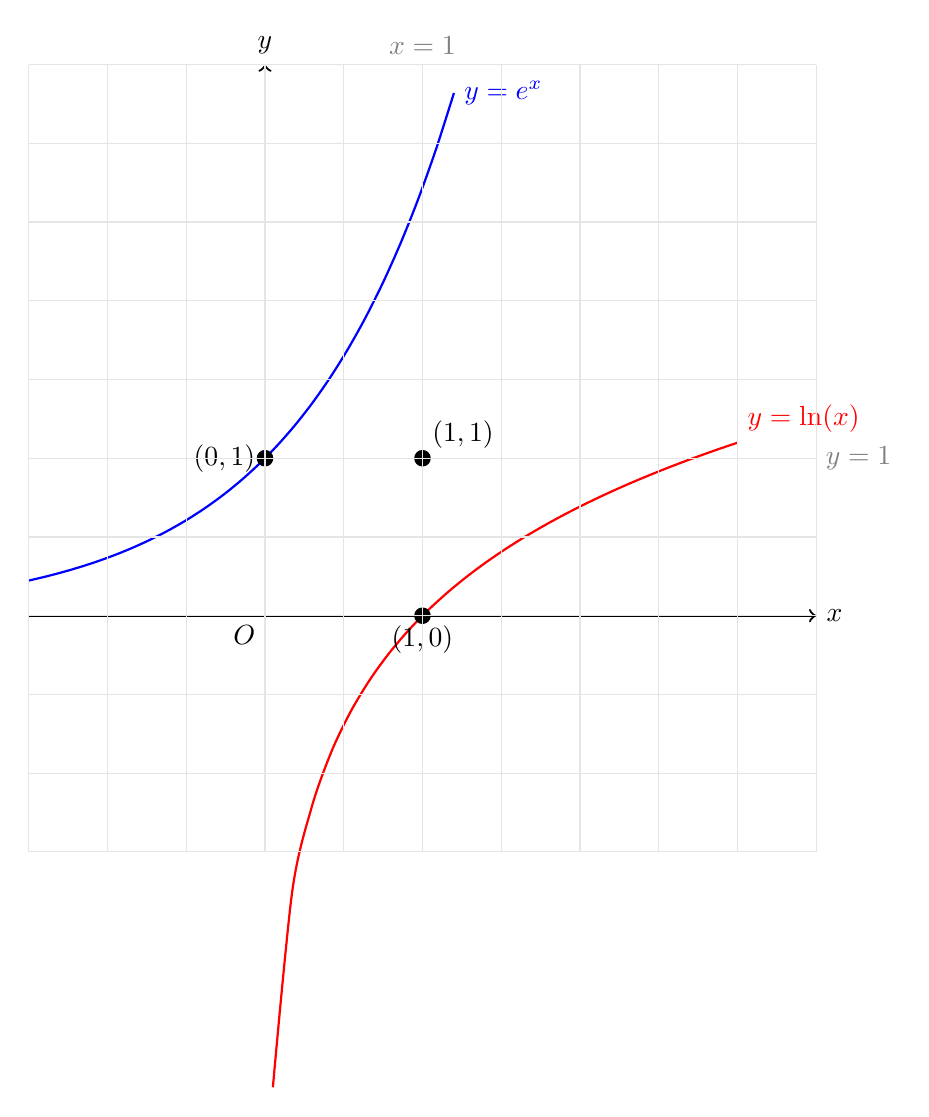
\begin{tikzpicture}[scale=2]


\draw[->, thick] (-1.5,0) -- (3.5,0) node[right] {$x$};
\draw[->, thick] (0,-1.5) -- (0,3.5) node[above] {$y$};
\draw[gray, dashed] (1,-1.5) -- (1,3.5) node[above] {$x=1$};
\draw[gray, dashed] (-1.5,1) -- (3.5,1) node[right] {$y=1$};


\node[below left] at (0,0) {$O$};


\draw[domain=-1.5:1.2, smooth, variable=\x, blue, thick] 
    plot ({\x}, {exp(\x)}) node[right] {$y = e^x$};


\draw[domain=0.05:3, smooth, variable=\x, red, thick] 
    plot ({\x}, {ln(\x)}) node[above right] {$y = \ln(x)$};

\fill[black] (0,1) circle (1.5pt) node[left] {$(0,1)$};
\fill[black] (1,0) circle (1.5pt) node[below] {$(1,0)$};
\fill[black] (1,1) circle (1.5pt) node[above right] {$(1,1)$};


\draw[gray!20, step=0.5] (-1.5,-1.5) grid (3.5,3.5);

\end{tikzpicture}
\end{document} 
